\documentclass[aspectratio=169]{beamer}

\graphicspath{{figures/}}

% Кириллица: pdfLaTeX -- через T2A, XeLaTeX/LuaLaTeX -- через системные шрифты.
\usepackage{iftex}
\ifPDFTeX
  \usepackage[T2A]{fontenc}
  \usepackage[utf8]{inputenc}
\else
  \usepackage{fontspec}
  \setsansfont{Arial}
\fi
\usepackage[english,russian]{babel}
\usepackage{amssymb,amsmath}
\usepackage{booktabs}

\usecolortheme{beaver}
\usefonttheme[onlymath]{serif}
\setbeamertemplate{navigation symbols}{}
\setbeamertemplate{footline}{}
\setbeamersize{text margin left=0.4cm,text margin right=0.4cm}
\setbeamerfont{frametitle}{size=\normalsize}

\title{CRISP: самоигра Challenger--Reasoner на основе корпуса документов}
\author{Роман Акрамов \quad Научный руководитель: Р.\,В.~Ищенко}
\date{}

\begin{document}

\begin{frame}{CRISP: вопросы из корпуса через самоигру улучшают сильную LLM,\\ а публичные math-датасеты её портят}
\vspace{-8pt}
\begin{columns}[T]
\begin{column}{0.31\textwidth}
\scriptsize
\textbf{Конвейер:} 766 PDF $\to$ OCR $\to$ корпус $\to$ самоигра $C \rightleftarrows R$ $\to$ LLM-судья $\to$ QA-датасет.

\smallskip
\textbf{Обозначения}
\begin{itemize}\setlength{\itemsep}{0pt}
  \item $C$ (Challenger) видит документ $d$, задаёт вопрос $q$ с ответом $a^*$
  \item $R$ (Reasoner) отвечает на $q$ \emph{без} $d$
  \item награда $C$: $r_C = \exp\!\bigl(-\tfrac{(\mathrm{Var}-0.25)^2}{0.02}\bigr)$, максимум при 50\% решаемости
  \item acc@1 --- доля верных ответов (avg@3, $T{=}0.6$)
\end{itemize}

\smallskip
\textbf{Эксперимент:} Qwen3-14B-Instruct, один рецепт GRPO на четырёх наборах данных, лучший чекпоинт по своему домену.
\end{column}
\begin{column}{0.67\textwidth}
\centering
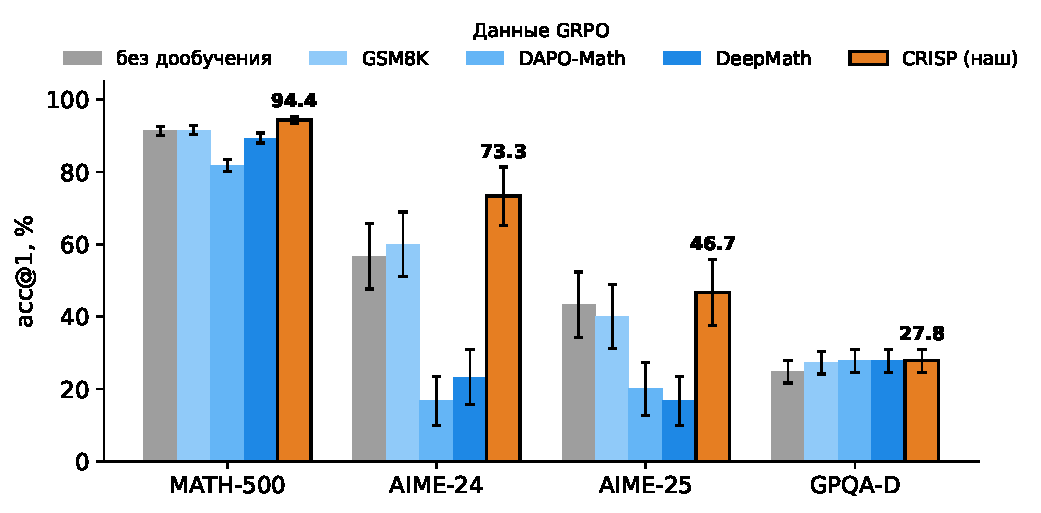
\includegraphics[width=0.94\textwidth]{oslide_main.pdf}\\[-2pt]
{\tiny Усы --- $\pm1$ std биномиального шума (AIME: 30 задач, MATH-500: 500, GPQA-D: 198).}

\vspace{3pt}
\begin{block}{Результат}
\scriptsize
GRPO на наших вопросах: MATH-500 $+3.0$, AIME-24 $+16.6$ п.п. к исходной модели;
GRPO на DAPO-Math и DeepMath роняет AIME на 23--40 п.п.
\end{block}
\end{column}
\end{columns}
\end{frame}

\end{document}
